\documentclass[10pt,twocolumn,letterpaper]{article}

\usepackage{cvpr}
\usepackage{times}
\usepackage{epsfig}
\usepackage{graphicx}
\usepackage{amsmath}
\usepackage{amssymb}

% Include other packages here, before hyperref.

% If you comment hyperref and then uncomment it, you should delete
% egpaper.aux before re-running latex.  (Or just hit 'q' on the first latex
% run, let it finish, and you should be clear).
\usepackage[pagebackref=true,breaklinks=true,letterpaper=true,colorlinks,bookmarks=false]{hyperref}

% \cvprfinalcopy % *** Uncomment this line for the final submission

\def\cvprPaperID{****} % *** Enter the CVPR Paper ID here
\def\httilde{\mbox{\tt\raisebox{-.5ex}{\symbol{126}}}}

% Pages are numbered in submission mode, and unnumbered in camera-ready
\ifcvprfinal\pagestyle{empty}\fi
\begin{document}

%%%%%%%%% TITLE
\title{Embracing Uncertainty: Coupling Cascaded Forest Predictors with
Model-based Marginals for Semantic Segmentation}

\author{First Author\\
Institution1\\
Institution1 address\\
{\tt\small firstauthor@i1.org}
% For a paper whose authors are all at the same institution,
% omit the following lines up until the closing ``}''.
% Additional authors and addresses can be added with ``\and'',
% just like the second author.
% To save space, use either the email address or home page, not both
\and
Second Author\\
Institution2\\
First line of institution2 address\\
{\tt\small secondauthor@i2.org}
}

\maketitle
%\thispagestyle{empty}

%%%%%%%%% ABSTRACT
\begin{abstract}
Embracing Uncertainty: Coupling Auto-context predictors with
Model-based Marginals for Spine Localization in Zebrafish

Embracing Uncertainty: Coupling Auto-context predictors with
Model-based Marginals for Semantic Segmentation

   We mix discriminative (discr) and generative models (gen), in a smart way.
\end{abstract}

%%%%%%%%% BODY TEXT
\section{Introduction}
The idea is to do "model-based smoothing" of the output of a Random Forest classifier, in an iterative or cascaded fashion.  This generalizes the idea proposed by GeoF~\cite{GeoForests2013}, which does "image aware" smoothing, using Geodesic distances. 
%
Another way to look at this is that we want to mix discriminative (discr) and generative models (gen), in a smart way.  E.g., The discr model initializes the gen model in the right search space, the gen model then refines this initialization.  This process is iterated while simultaneously increasing the "confidence" in the discr model output. 

Our contributions: 
%
(1) Use Active Appearance Model and HMM for "`image aware"' smoothing in a RF cascade. 
Closest works: 
First, AutoContext~\cite{AutoContext2008}, but they don't do any smoothing. 
Second, GeoF~\cite{GeoForests2013}, but they don't use a generative model for smoothing. 
Third, Glocker~\cite{Glocker2013}, but they do not run a cascade. 
%
(2) Tree weighting based on smoothing. Can be combined with any kind of smoothing. Idea: rate the trees of a forest: who agrees most with the smoothed output? This way, ...
%


Literature.

---- SSMs and Random Forests:

Cootes Femur TMI 2013~\cite{CootesFemurTMI2013}

Cootes Regression Forest + SSM ECCV 2012~\cite{CootesECCV2012RRFandSSM}

---- Constellation models and Forests:

Spine: Glocker~\cite{Glocker2013}

Body parts: Auto Context~\cite{AutoContext2008}, "`Pose Machines"' ECCV 2014~\cite{PoseMachinesECCV2014}

Abdominal images: GeoF~\cite{GeoForests2013}, and GeoF at IPMI 2011~\cite{CriminisiAbdominalIPMI2011}: "'Entangled Decision Forests and their Application for Semantic Segmentation of CT Images"'. Seifert SPIE: Marginal space learning classifier plus MRF~\cite{SeifertAnatomicalSPIE2009} 

(Fish: Rotation invariant features, Ronneberger VibeZ)

---- Cascading with Model Fit

DTF, RTF, GeoF

---- Constellation models of self-similar structures

Spine: (Glocker) Klinder (SSM)~\cite{Klinder2009471}: Generalized Hough Transform as detector

Dental: our MICCAI 2012~\cite{TeethMICCAI2012} (Generalized Hough Transform + SSM as detector)

Worm~\cite{WormMiccai2014}

\section{Background}

\subsection{RF}
Filter Bank, Classification Forest, offset and difference features. 

\paragraph{Cascade}

\paragraph{Constellation Model/Inference}
HMM, probabilistic inference.

\subsection{AAM}
Active appearance models (AAMs)~\cite{CootesAAM2001} are linear, generative, parametric models of shape and appearance that are learned (PCA) from training data.  Fitting an AAM is a non-linear optimisation problem, that is done via incremental updates to fitting parameters.  Importantly, AAMs can be easily extended to include priors on the model parameters (see also~\cite{BakerAAM2004}).  

Shape Model:

\[s = s_0 + \sum_{i=1}^n p_i s_i\]

where s is a vector of x,y coordinates of the landmarks that define the shape.  From PCA, $s_0$ is the mean shape, and $s_i$ are n eigenvectors corresponding to the n largest eigenvalues.  Not shown here is that the training data is first noramlised using a Procrustes analysis using a global shape normalising transformation (in our case, a similarity transform) to avoid modeling this variation in the linear model.

Appearance Model:

\[A(x) = A_0(x) + \sum_{i=1}^m \lambda_i A_i(x)\]

Analogous to shape model. $A_0$ and $A_i$ are computed from PCA on a set of \emph{shape normalised} training images, which have been warped onto the base-mesh $s_0$.  Shape normalizing is a key benefit of AAMs (compared to e.g. Eigen-faces), and leads to more compressed PCA representation.

To create a model instance, create an image A(x) (defined by $\lambda$) on the base-mesh, and then warp it to s (defined by p).  Warping is done using a thin-plate spline, parameterized by the set of landmarks, $s_0$ and s.  This defines the unique warp parameterised by p, called W(x;p).

Fitting criteria:

\[Error = A_0(x) + \sum_{i=1}^m \lambda_i A_i(x) - I(N(W(x;p);q)) \]

where N(x;q) is the similarity transform, parameterized by q, and the cost is typically the sum of squared errors over the shape normalized patch.

\[Cost = \sum_{x \epsilon s_0} [Error]^2 \]

Final note, the most efficient fitting routine [] actually "projects out" the appearance variation (from the Error image), and simply solves for the parameters of the transformation: p,q.  If you keep one shape parameter (n=1), this leads to a 5 parameter model.

\paragraph{Priors}

One can add priors on the model parameters, as follows:

\[ \sum_{x \epsilon s_0} [A(x) - I(N(W(x;p);q)]^2 + \sum_{i=1}^K F_i^2(p,q) \]

If $F_i(p,q)$ is quadratic, this can be interpreted in the Bayesian framework as Gaussian Regularization.  There's also a clear way to "ramp" the importance of the priors as:

\[ F_i^2(p,q) = r[(p-p_0)^2+(q-q_0)^2]) \]

where r is the parameter that captures how much we trust the discr model output (this could be learned).

Note, adding priors doesn't slow down the code too much.  You can still use the same fitting algorithm, there's just some extra computation in each loop.


\section{Method: Cascaded RF Interleaved with Probabilistic Generative Constellation Model Inference}

By the above method, a number of model instances would be initialized and fit, for each segment.  Each model instance has a cost associated with its fit.  Use these costs as unaries in a Markov Chain Model.  The pair-wise energy comes from statistics on the relative position of neighboring segments in the training data.  This is exactly what Glocker did already; however, we would do probabilistic inference (rather than MAP inference) and keep all the marginals.

\subsection{We get Two Results: RF Output, smoothed Output.}

\subsection{Tree Weights?}

\section{Results}
Approach: Cascade interleaved with "`smoothing"'. 
Evaluation: Different kinds of "`smoothing"', each with different kinds of outputs.

Dataset: 32 images of developing zebrafish. Task: Semantic segmentation of 21 somites (i.e.\ developing vertebrae).

\paragraph{Our Setup: Probabilistic Inference}

\paragraph{Comparison: Auto Context}

\paragraph{Comparison: GeoF}

\paragraph{Comparison: MAP Inference}

Experiments:
\begin{enumerate}
\item Auto Context
\item GeoF (two versions)
\item AAM with MAP inference 
\item AAM with probabilistic inference 
\item (AAM with probabilistic inference, tree weighting)
\end{enumerate}

\begin{figure}[t]
\begin{center}
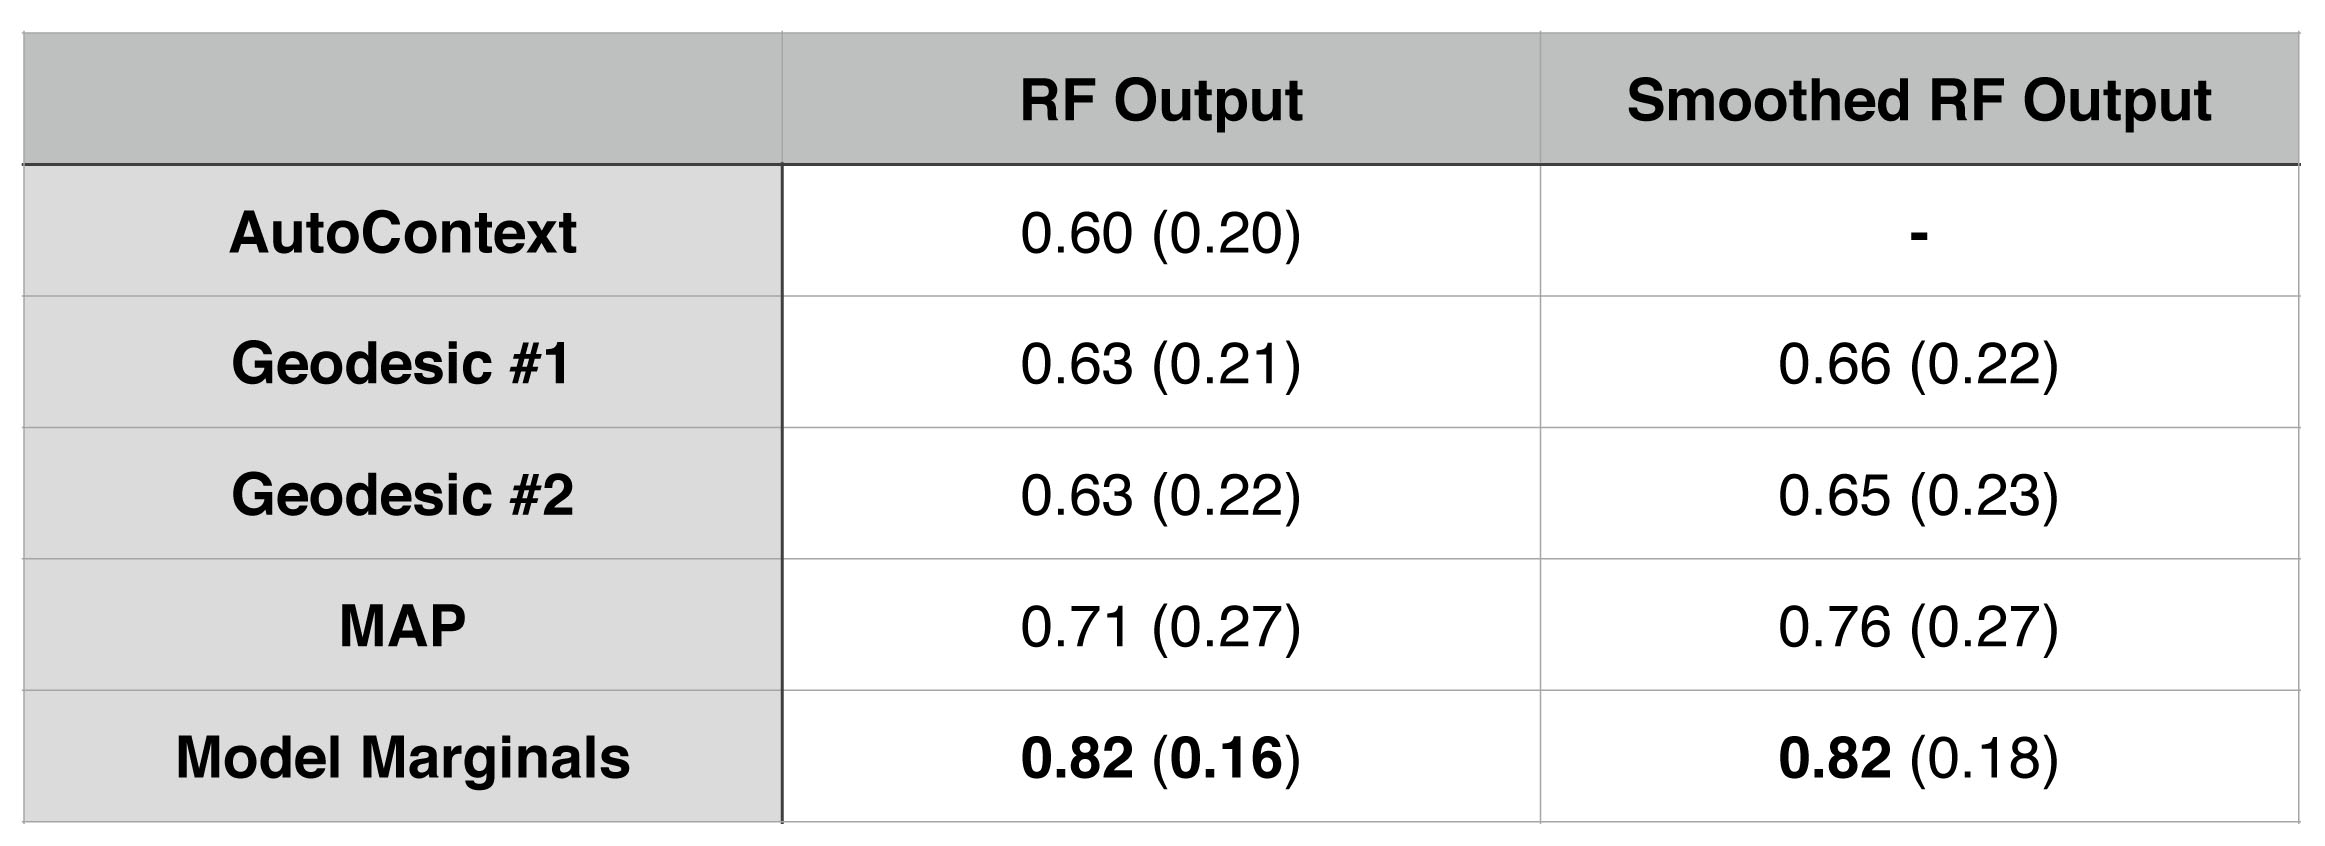
\includegraphics[width=\columnwidth]{TableDiceScores.jpg} %&[trim=0cm 2cm 0cm 1cm,height=0.2\textheight]
\caption{Evaluation on 32 datasets. Dice Scores on all 21 Somites: Mean and standard deviation (in brackets).}
\label{tab:results}
\end{center}
\end{figure}

\begin{figure*}[tb]
\centering
\small
\begin{center}
%	\figpart{a}
		(a) \includegraphics[trim=0cm 2cm 0cm 1cm,height=0.2\textheight]{gfx/boxplot_RF.png} %&
%	\quad
%	\figpart{b}
		(b) \includegraphics[trim=.75cm 2cm 0cm 1cm,height=0.2\textheight]{gfx/boxplot_GeoF.png} \\
%	\,
%	\figpart{c}
		(c) \includegraphics[trim=.75cm 2cm 0cm 1cm,height=0.2\textheight]{gfx/boxplot_model.png} %\\
\end{center}
%\includegraphics[trim=4cm 0cm 5cm 0cm, clip=true, width=0.45\textwidth]{gfx/noInpainting.png} \\
\label{boxplots}
% \vspace{-2mm}
\caption{ %Box plots of Dice scores.}
%\figpart{a}~ 
(a) 2 level cascade, RF output 
%
% \figpart{b}~
(b) geodesic smoothing, 1st level
%
% \figpart{c}~
(c) model fit}
\end{figure*}

\section{Discussion}
Ours is the best :)

\paragraph{Cascading Helps!}
... performance goes up over levels. Boxplots!

... "`traditional"' MAP after one level sucks. 

\paragraph{Smoothing Helps! Model-based Smoothing Helps Best!}
... Auto Context $<$ GeoF $<$ Model Based. Reason: More Specific Prior knowledge...

\paragraph{Uncertainty Helps!}
... Probabilistic inference considerably outperforms MAP inference (6\% better). Reason: With Prob.\ inference, cases can be rescued if not caught after first level (i.e.\ "`at first site"'). Show some rescue cases. 

We also tried MAP after third level. Once all cases are rescued, MAP is fine (performs equally -- state numbers). BUT NOT EARLIER!



\section{Overview of Idea}

The initial idea is to do "model-based smoothing" of the output of a Random Forest classifier, in an iterative or cascaded fashion.  This generalizes the idea proposed by GeoF, which does "image aware" smoothing, using Geodesic distances.  Another potential contribution is the idea of learning the smoothing parameter.  Intuitively, it seems like the smoothing should be most active in the early stages of the cascade, when the output is most dubious, and then should decrease as you trust the output more with each iteration.

Another way to look at this is that we want to mix discriminative (discr) and generative models (gen), in a smart way.  E.g., The discr model initializes the gen model in the right search space, the gen model then refines this initialization.  This process is iterated while simultaneously increasing the "confidence" in the discr model output.

Oddly, when thinking about this, it seems like the choice of discr model to use is sensitive to the above statement of purpose.  For example, GeoF uses classification, which provides a suitable output (a probability map) for smoothing.  However, the transition between discr and gen models is more seamless when the parameters of the model are regressed directly.  I'll return to this point.

\section{Related work}

\begin{enumerate}
\item GeoF~\cite{GeoForests2013}: Geodesic smoothing of RF output.  Uses an Entangled Forest.
\item Deformable Templates Guided Discriminative Models for Robust 3D Brain MRI Segmentation.~\cite{BrainSeg2013}  Liu et al.  2013: Uses generative model to "refine" features in a cascaded discriminative classifier.
\item AutoContext~\cite{AutoContext2008}.  Tu.  2008.
\item Automatic Localization and Identification of Vertebrae in Arbitrary Field-of-View CT Scans.~\cite{Glocker2012} Glocker et al.  2012: Uses Regression Forest.
\item Vertebrae Localization in Pathological Spine CT via Dense Classification from Sparse Annotations.~\cite{Glocker2013} Glocker et al.  2013: Uses Classification this time.
\item Uwe's hint \cite{Denzler2012}: As Time Goes by -- Anytime Semantic Segmentation with Iterative Context Forests
\end{enumerate}
* List is still in progress


\section{Classification-based Approach}

I'll first describe an approach using an RF classifier as the descr function.  Then I'll compare and contrast how it might look using RF regression as the descr function.

\subsection{Random Forest Classifier}

Currently, I use an RF classifier with roughly 50 features calculated from the grayscale image.  Importantly, 2 of these features are the XY position, which introduces some global "context" early on.  (For this to work, I align the images based on masks that I compute using Sbalzarini's near-optimal thresholding algorithm).  Other features include standard filter-bank responses, from which I select the 50 best using variable importance.

If one were to do cascading without any smoothing, it would be very similar to AutoContext.  This is implemented by extending the number of features in the feature stack to include the posterior probabilities of each class (i.e. the RF output, with one new feature for each class).  In the first iteration, these probabilities are all uniform, so the decision trees ignore them, because they're non-descriminating.  After each iteration, these probability maps are updated with the output of the previous forest.

I would propose to follow the GeoF method and keep the raw RF output when introducing the smoothed prob maps.  In this case, just add (again) one new feature for each class, but this time corresponding to the smoothed RF output.  In the first iteration, these prob maps are also uniform.  In subsequent iterations, they're updated by the smoothed output of the previous forest.  Altogether, this is roughly 100 features: 50 from filter responses, 25 from RF output, 25 from smoothed RF output.

A few technical notes: VIGRA introduces randomization both through bagging (every tree sees a random subset of the data), and random node optimization (every node optimizes over a random subset of the features).  Context can then be introduced by allowing nodes to select features with a randomly selected offset from their current location.  Note: autocontext only allows non-local feature selection in the subset of "probability features" (meaning RF output).  I haven't found a good justification for this, so would probably allow non-local selection for all features.

\section{Model-based Smoothing of RF Output}

The first step is to use the AAM model to fit the grayscale image in a way that is guided by the output of the RF.  There are (at least) two ways to do this: additive and multiplicative.

\subsection{Additive Method}

Simultaneously minimize the error from two AAMs:

\[ \sum_{x \epsilon s_0} [A(x) - I(N(W(x;p);q)]^2 + r\sum_{x \epsilon s_0} [A_2(x) - I_2(N(W(x;p);q)]^2 \]

where $I_2$ is the RF output and $A_2(x)$ is a "soft mask" from averaging all of the ground truth labelings.  Again, r weights the relative importance of the two terms.  I would tend not to include linear appearance variation for the mask, and since the warp parameters are the same as for the original grayscale image, this doesn't introduce any new AAM parameters.

\subsection{Multiplicative Method}

The most efficient optimization method actually proceeds by minizing the following expression, with respect to $\Delta p$ and $\Delta q$:

\[ \sum_{x \epsilon s_0} [A(N(W(x;\Delta p);\Delta q) - I(N(W(x;p);q)]^2 \]

Thus, I think one can introduce the following change, without breaking the optimization algorithm:

\[ \sum_{x \epsilon s_0} [I_3(N(W(x;p);q)]*[A(N(W(x;\Delta p);\Delta q) - I(N(W(x;p);q)]^2 \]

where $I_3 = 1 - r*log(p(c))$, r is again the relative importance parameter, and p(c) is the prob of class c at pixel x.  This is analogous to using a Robust statistic, which is a per-pixel weight; however, it's a bit more complicated, since the mask of weights is dependent on the warp itself, and so needs to updated during fitting.  This suggests it could be a good deal slower to do the fitting (which is true for Robust Stats).

\subsection{Inference on the Whole Spine}


\subsection{Generating a Smoothed RF Output}

The simplest way to generate a smoothed RF Output is to re-use the Geodesic smoothing idea from Criminisi.  Let:

\[ Q(x; M, \nabla I) = \min_{x'} (\delta (x,x') + \nu M) \]

and $\nu$ is some free parameter.  Note, x and x' are two points in the image. $M(x') = 1 - p(c|v(x'))$, where v(x') is the feature vector at pixel x'.  Then the smoothed RF output is calculated as:

\[ g(c|v(x)) = \frac{1}{Z} p(c|v(x)) e^{\frac{-Q(x;p(c|v(\Omega)),\nabla J)^2}{\sigma ^2}} \]

This accomplishes smoothing in quite an indirect way, as a competition between different possible class labels for a given pixel, mediated by the normalization Z.  \textbf{It would be interesting to think of more direct ways to implement smoothing.}  However, within this framework, we could just replace the geodesic distance function and the definition of M.

Recall, since we initialized many AAMS for fitting, and did probabilistic inference over all of these solutions, we have multiple masks each with its own probability.  I would propose to use a distance function from each instance \emph{s} of the AAM model fits.

\[ \delta (x,s) = \begin{cases} 0, & \mbox{if } x \epsilon \Omega _s \\ d(x, \Omega _s), & \mbox{else} \end{cases} \]

\[ d(x,\Omega _s) = \inf_{y \epsilon \Omega _s} d(x,y) \]

where $\Omega _s$ is the mask associated with instance s.  Then, 

\[ M(s) = 1 - p(s) \] 

\[ Q(x; M(s), \nabla I) = \min_{s} (\delta (x,s) + \nu M(s)) \]

where p(s) is the probability of a given model instance.  The intuition is as follows: If a pixel x is within the mask region corresponding to a highly probable AAM model fit, then it keeps it's probability; however, if it's far from one of these regions, then it's probability would be reduced.  Through the renormalization, this accomplishes the desired smoothing, as in GeoF.

\subsection{Feature Generation vs. Smoothing}

An alternative way to generate an output from the above method, to be fed back into another RF, is to simply "stamp" the masks associated with the above model instances into an image.  This would amount to a weighted average.

\[ p(c) = \sum_{s=1}^S p(c|s)p(s) \]

where there are S model instances initialized, $p(c|s)$ is a mask associated with model instance s, and p(s) is the prob of model instance s from the probilistic inference.

This "stamping" approach is similar to the smoothing above, except it's not mixed with the original RF output.  From the perspective of generating useful features, this seems like an OK idea.  Question: Is smoothing inherently better than this approach?

\subsection{Parameters}

\begin{itemize}
\item n: \# of shape modes
\item m: \# of appearance modes
\item r: trust in discr output
\item S: \# of model instances that are initialized for fitting
\item g: \# of grad descent steps
\end{itemize}

all parameters could potentially ramp with increasing depth in the cascade to reflect increasing confidence that the model starts in a good search space.  r is potentially most interesting.

\subsection{Objective Function and Learning}

The most trivial approach is to simply do a line search over the free parameters. For example, taking r from above as a free parameter, it can be set at each level of the cascade. One way to do this is greedy optimization at every stage.  This is already done within the RFs, which optimize each node independently.  One could then optimize the parameters of the AAM fit (e.g., r) to give the best output of the next forest, with respect to some loss function.  A reasonable loss function is:

\[ \sum_{x \epsilon \Omega} [l(x) \neq c(x)] w(c(x)) \]

with,

\[ w(c) = \frac{1}{\sum_{x \epsilon \Omega} [c(x) = c]} \]

One nice feature is that the learning is then independent of the number of levels in the cascade.

Rather than an exhaustive search over the free parameters, it would be much nicer to learn them using standard approaches of gradient descent.  Is this possible?  This would be a really nice contribution, if one could show how to do this using e.g., back-prop...

\subsection{Model Initialisation}

A key aspect of the problem is how to initialize the AAM model for fitting.  This is one of the big challenges of AAMs, since they're local search methods, and a big benefit of using the RF.  However, there doesn't seem to be a "nice" way to initialize the AAM directly from the RF output.  It's easy to think of ways to initialize the XY position directly from the RF output, but how should you initialize orientation, scale, shape, appearance?  There are for sure some \emph{ad hoc} ways, but it doesn't feel very elegant.  This is where it's interesting to contrast regression, which directly gives you the initialization.

\section{Regression-based Approach}

In the framework of inter-twining gen and discr models, regression seems much better suited than classification, because it operates on the same set of variables as the gen model.  The one big downside is the number of variables to be regressed could be quite large.  For example, in classification I have 22 classes (including background).  In regression, I would have 21x5 variables to regress (way too many!).  Rather I would need to build my AAM differently, not from individual units, but rather from the whole spine.  My guess is that this would greatly reduce the number of parameters (to 10?), but it would also give up a lot of freedom.  In particular, I would need a completely new spine model for each developmental stage.

\subsection{Initialization and Priors}

Obviously, using a regression RF would directly give me the initialization of all my gen model variables.  Additionally, from the point cloud of regressed parameters (where each pixel contributes one point to the cloud), I could estimate a distribution and feed this in as priors on the parameters.  This should naturally display the correct behaviour, that as the regression improves, the priors would become stronger and stabilize the AAM fitting.

\subsection{Feature Generation}

The link between discr and gen models still seems to break down when transitioning from the gen model back to the discr model.  To make the cycle "complete", one would need to use Conditional Regression Forests, which store global latent variables. Then you could go directly back and forth between regressing the global parameters, refining them via gen model fitting, and using the refined values for the next round of estimation (regression).  This seems really beautiful!  Has it been done before?  If not, could we think of a simple test case with only a few model parameters to demonstrate this idea?

Alternatively, we can use the same "stamping" technique described in the classification RF cascade.  Given the final fitting parameters of the gen model, generate the corresponding image, and feed this back to the next RF as a new feature.  Do this for every segment.  The only difference to classification is that you get grayscale images, rather than probability images.

\textbf{Comment:} It's not clear if the new "stamped" features that are returned from the gen model are as useful in the case of regression as they were in the case of classification.  The class probabilities condense a lot of information, and are likely much richer features.









\section{Introduction}

Please follow the steps outlined below when submitting your manuscript to
the IEEE Computer Society Press.  This style guide now has several
important modifications (for example, you are no longer warned against the
use of sticky tape to attach your artwork to the paper), so all authors
should read this new version.

%-------------------------------------------------------------------------
\subsection{Language}

All manuscripts must be in English.

\subsection{Dual submission}

Please refer to the author guidelines on the CVPR 2015 web page for a
discussion of the policy on dual submissions.

\subsection{Paper length}
For CVPR 2015, the rules about paper length have changed, so please
read this section carefully. Papers, excluding the references section,
must be no longer than eight pages in length. The references section
will not be included in the page count, and there is no limit on the
length of the references section. For example, a paper of eight pages
with two pages of references would have a total length of 10 pages.
{\bf Unlike previous years, there will be no extra page charges for
  CVPR 2015.}

Overlength papers will simply not be reviewed.  This includes papers
where the margins and formatting are deemed to have been significantly
altered from those laid down by this style guide.  Note that this
\LaTeX\ guide already sets figure captions and references in a smaller font.
The reason such papers will not be reviewed is that there is no provision for
supervised revisions of manuscripts.  The reviewing process cannot determine
the suitability of the paper for presentation in eight pages if it is
reviewed in eleven.  

%-------------------------------------------------------------------------
\subsection{The ruler}
The \LaTeX\ style defines a printed ruler which should be present in the
version submitted for review.  The ruler is provided in order that
reviewers may comment on particular lines in the paper without
circumlocution.  If you are preparing a document using a non-\LaTeX\
document preparation system, please arrange for an equivalent ruler to
appear on the final output pages.  The presence or absence of the ruler
should not change the appearance of any other content on the page.  The
camera ready copy should not contain a ruler. (\LaTeX\ users may uncomment
the \verb'\cvprfinalcopy' command in the document preamble.)  Reviewers:
note that the ruler measurements do not align well with lines in the paper
--- this turns out to be very difficult to do well when the paper contains
many figures and equations, and, when done, looks ugly.  Just use fractional
references (e.g.\ this line is $095.5$), although in most cases one would
expect that the approximate location will be adequate.

\subsection{Mathematics}

Please number all of your sections and displayed equations.  It is
important for readers to be able to refer to any particular equation.  Just
because you didn't refer to it in the text doesn't mean some future reader
might not need to refer to it.  It is cumbersome to have to use
circumlocutions like ``the equation second from the top of page 3 column
1''.  (Note that the ruler will not be present in the final copy, so is not
an alternative to equation numbers).  All authors will benefit from reading
Mermin's description of how to write mathematics:
\url{http://www.pamitc.org/documents/mermin.pdf}.


\subsection{Blind review}

Many authors misunderstand the concept of anonymizing for blind
review.  Blind review does not mean that one must remove
citations to one's own work---in fact it is often impossible to
review a paper unless the previous citations are known and
available.

Blind review means that you do not use the words ``my'' or ``our''
when citing previous work.  That is all.  (But see below for
techreports.)

Saying ``this builds on the work of Lucy Smith [1]'' does not say
that you are Lucy Smith; it says that you are building on her
work.  If you are Smith and Jones, do not say ``as we show in
[7]'', say ``as Smith and Jones show in [7]'' and at the end of the
paper, include reference 7 as you would any other cited work.

An example of a bad paper just asking to be rejected:
\begin{quote}
\begin{center}
    An analysis of the frobnicatable foo filter.
\end{center}

   In this paper we present a performance analysis of our
   previous paper [1], and show it to be inferior to all
   previously known methods.  Why the previous paper was
   accepted without this analysis is beyond me.

   [1] Removed for blind review
\end{quote}


An example of an acceptable paper:

\begin{quote}
\begin{center}
     An analysis of the frobnicatable foo filter.
\end{center}

   In this paper we present a performance analysis of the
   paper of Smith \etal [1], and show it to be inferior to
   all previously known methods.  Why the previous paper
   was accepted without this analysis is beyond me.

   [1] Smith, L and Jones, C. ``The frobnicatable foo
   filter, a fundamental contribution to human knowledge''.
   Nature 381(12), 1-213.
\end{quote}

If you are making a submission to another conference at the same time,
which covers similar or overlapping material, you may need to refer to that
submission in order to explain the differences, just as you would if you
had previously published related work.  In such cases, include the
anonymized parallel submission~\cite{Authors14} as additional material and
cite it as
\begin{quote}
[1] Authors. ``The frobnicatable foo filter'', F\&G 2014 Submission ID 324,
Supplied as additional material {\tt fg324.pdf}.
\end{quote}

Finally, you may feel you need to tell the reader that more details can be
found elsewhere, and refer them to a technical report.  For conference
submissions, the paper must stand on its own, and not {\em require} the
reviewer to go to a techreport for further details.  Thus, you may say in
the body of the paper ``further details may be found
in~\cite{Authors14b}''.  Then submit the techreport as additional material.
Again, you may not assume the reviewers will read this material.

Sometimes your paper is about a problem which you tested using a tool which
is widely known to be restricted to a single institution.  For example,
let's say it's 1969, you have solved a key problem on the Apollo lander,
and you believe that the CVPR70 audience would like to hear about your
solution.  The work is a development of your celebrated 1968 paper entitled
``Zero-g frobnication: How being the only people in the world with access to
the Apollo lander source code makes us a wow at parties'', by Zeus \etal.

You can handle this paper like any other.  Don't write ``We show how to
improve our previous work [Anonymous, 1968].  This time we tested the
algorithm on a lunar lander [name of lander removed for blind review]''.
That would be silly, and would immediately identify the authors. Instead
write the following:
\begin{quotation}
\noindent
   We describe a system for zero-g frobnication.  This
   system is new because it handles the following cases:
   A, B.  Previous systems [Zeus et al. 1968] didn't
   handle case B properly.  Ours handles it by including
   a foo term in the bar integral.

   ...

   The proposed system was integrated with the Apollo
   lunar lander, and went all the way to the moon, don't
   you know.  It displayed the following behaviours
   which show how well we solved cases A and B: ...
\end{quotation}
As you can see, the above text follows standard scientific convention,
reads better than the first version, and does not explicitly name you as
the authors.  A reviewer might think it likely that the new paper was
written by Zeus \etal, but cannot make any decision based on that guess.
He or she would have to be sure that no other authors could have been
contracted to solve problem B.

FAQ: Are acknowledgements OK?  No.  Leave them for the final copy.


\begin{figure}[t]
\begin{center}
\fbox{\rule{0pt}{2in} \rule{0.9\linewidth}{0pt}}
   %\includegraphics[width=0.8\linewidth]{egfigure.eps}
\end{center}
   \caption{Example of caption.  It is set in Roman so that mathematics
   (always set in Roman: $B \sin A = A \sin B$) may be included without an
   ugly clash.}
\label{fig:long}
\label{fig:onecol}
\end{figure}

\subsection{Miscellaneous}

\noindent
Compare the following:\\
\begin{tabular}{ll}
 \verb'$conf_a$' &  $conf_a$ \\
 \verb'$\mathit{conf}_a$' & $\mathit{conf}_a$
\end{tabular}\\
See The \TeX book, p165.

The space after \eg, meaning ``for example'', should not be a
sentence-ending space. So \eg is correct, {\em e.g.} is not.  The provided
\verb'\eg' macro takes care of this.

When citing a multi-author paper, you may save space by using ``et alia'',
shortened to ``\etal'' (not ``{\em et.\ al.}'' as ``{\em et}'' is a complete word.)
However, use it only when there are three or more authors.  Thus, the
following is correct: ``
   Frobnication has been trendy lately.
   It was introduced by Alpher~\cite{Alpher02}, and subsequently developed by
   Alpher and Fotheringham-Smythe~\cite{Alpher03}, and Alpher \etal~\cite{Alpher04}.''

This is incorrect: ``... subsequently developed by Alpher \etal~\cite{Alpher03} ...''
because reference~\cite{Alpher03} has just two authors.  If you use the
\verb'\etal' macro provided, then you need not worry about double periods
when used at the end of a sentence as in Alpher \etal.

For this citation style, keep multiple citations in numerical (not
chronological) order, so prefer \cite{Alpher03,Alpher02,Authors14} to
\cite{Alpher02,Alpher03,Authors14}.


\begin{figure*}
\begin{center}
\fbox{\rule{0pt}{2in} \rule{.9\linewidth}{0pt}}
\end{center}
   \caption{Example of a short caption, which should be centered.}
\label{fig:short}
\end{figure*}

%------------------------------------------------------------------------
\section{Formatting your paper}

All text must be in a two-column format. The total allowable width of the
text area is $6\frac78$ inches (17.5 cm) wide by $8\frac78$ inches (22.54
cm) high. Columns are to be $3\frac14$ inches (8.25 cm) wide, with a
$\frac{5}{16}$ inch (0.8 cm) space between them. The main title (on the
first page) should begin 1.0 inch (2.54 cm) from the top edge of the
page. The second and following pages should begin 1.0 inch (2.54 cm) from
the top edge. On all pages, the bottom margin should be 1-1/8 inches (2.86
cm) from the bottom edge of the page for $8.5 \times 11$-inch paper; for A4
paper, approximately 1-5/8 inches (4.13 cm) from the bottom edge of the
page.

%-------------------------------------------------------------------------
\subsection{Margins and page numbering}

All printed material, including text, illustrations, and charts, must be kept
within a print area 6-7/8 inches (17.5 cm) wide by 8-7/8 inches (22.54 cm)
high.



%-------------------------------------------------------------------------
\subsection{Type-style and fonts}

Wherever Times is specified, Times Roman may also be used. If neither is
available on your word processor, please use the font closest in
appearance to Times to which you have access.

MAIN TITLE. Center the title 1-3/8 inches (3.49 cm) from the top edge of
the first page. The title should be in Times 14-point, boldface type.
Capitalize the first letter of nouns, pronouns, verbs, adjectives, and
adverbs; do not capitalize articles, coordinate conjunctions, or
prepositions (unless the title begins with such a word). Leave two blank
lines after the title.

AUTHOR NAME(s) and AFFILIATION(s) are to be centered beneath the title
and printed in Times 12-point, non-boldface type. This information is to
be followed by two blank lines.

The ABSTRACT and MAIN TEXT are to be in a two-column format.

MAIN TEXT. Type main text in 10-point Times, single-spaced. Do NOT use
double-spacing. All paragraphs should be indented 1 pica (approx. 1/6
inch or 0.422 cm). Make sure your text is fully justified---that is,
flush left and flush right. Please do not place any additional blank
lines between paragraphs.

Figure and table captions should be 9-point Roman type as in
Figures~\ref{fig:onecol} and~\ref{fig:short}.  Short captions should be centred.

\noindent Callouts should be 9-point Helvetica, non-boldface type.
Initially capitalize only the first word of section titles and first-,
second-, and third-order headings.

FIRST-ORDER HEADINGS. (For example, {\large \bf 1. Introduction})
should be Times 12-point boldface, initially capitalized, flush left,
with one blank line before, and one blank line after.

SECOND-ORDER HEADINGS. (For example, { \bf 1.1. Database elements})
should be Times 11-point boldface, initially capitalized, flush left,
with one blank line before, and one after. If you require a third-order
heading (we discourage it), use 10-point Times, boldface, initially
capitalized, flush left, preceded by one blank line, followed by a period
and your text on the same line.

%-------------------------------------------------------------------------
\subsection{Footnotes}

Please use footnotes\footnote {This is what a footnote looks like.  It
often distracts the reader from the main flow of the argument.} sparingly.
Indeed, try to avoid footnotes altogether and include necessary peripheral
observations in
the text (within parentheses, if you prefer, as in this sentence).  If you
wish to use a footnote, place it at the bottom of the column on the page on
which it is referenced. Use Times 8-point type, single-spaced.


%-------------------------------------------------------------------------
\subsection{References}

List and number all bibliographical references in 9-point Times,
single-spaced, at the end of your paper. When referenced in the text,
enclose the citation number in square brackets, for
example~\cite{Authors14}.  Where appropriate, include the name(s) of
editors of referenced books.

\begin{table}
\begin{center}
\begin{tabular}{|l|c|}
\hline
Method & Frobnability \\
\hline\hline
Theirs & Frumpy \\
Yours & Frobbly \\
Ours & Makes one's heart Frob\\
\hline
\end{tabular}
\end{center}
\caption{Results.   Ours is better.}
\end{table}

%-------------------------------------------------------------------------
\subsection{Illustrations, graphs, and photographs}

All graphics should be centered.  Please ensure that any point you wish to
make is resolvable in a printed copy of the paper.  Resize fonts in figures
to match the font in the body text, and choose line widths which render
effectively in print.  Many readers (and reviewers), even of an electronic
copy, will choose to print your paper in order to read it.  You cannot
insist that they do otherwise, and therefore must not assume that they can
zoom in to see tiny details on a graphic.

When placing figures in \LaTeX, it's almost always best to use
\verb+\includegraphics+, and to specify the  figure width as a multiple of
the line width as in the example below
{\small\begin{verbatim}
   \usepackage[dvips]{graphicx} ...
   \includegraphics[width=0.8\linewidth]
                   {myfile.eps}
\end{verbatim}
}


%-------------------------------------------------------------------------
\subsection{Color}

Please refer to the author guidelines on the CVPR 2015 web page for a discussion
of the use of color in your document.

%------------------------------------------------------------------------
\section{Final copy}

You must include your signed IEEE copyright release form when you submit
your finished paper. We MUST have this form before your paper can be
published in the proceedings.

Please direct any questions to the production editor in charge of these
proceedings at the IEEE Computer Society Press: Phone (714) 821-8380, or
Fax (714) 761-1784.

{\small
\bibliographystyle{ieee}
\bibliography{somites2014}
}

\end{document}
